\chapter{Design}

\section{Introduction}

\subsection{Purpose}
This software design document describes the architecture and system design of Forensics Linguistics and Authorship Attribution using Stylometry.

\subsection{Scope}
The project is intended to create a system for parsing and analyzing text for the extraction of linguistic and stylometric features to be used in authorship attribution performed by linguistic analysts.

\subsubsection{Goals}
\begin{itemize}
    \item Reduce analysis time.
    \item Ease exploration of new features.
    \item Authorship attribution.
\end{itemize}

\subsubsection{Objectives}
\begin{itemize}
    \item Intuitive interface.
    \item Bulk analysis.
    \item Features management.
    \item Analysis modification.
    \item Statistical and methods for authorship attribution.
\end{itemize}

\subsection{Overview}
The system is meant to be used by linguistic professionals to extract features from text and receive a preliminary analysis on the whole corpus' author.

\section{System Overview}
The system will receive the corpus from the user in the form of a compressed file, and the features required for extraction, which will then be processed for the required output and analyzed for a disputed text if necessary.

\section{System Architecture}

\subsection{Architectural Design}
\begin{figure}[tbh]
    \centering
    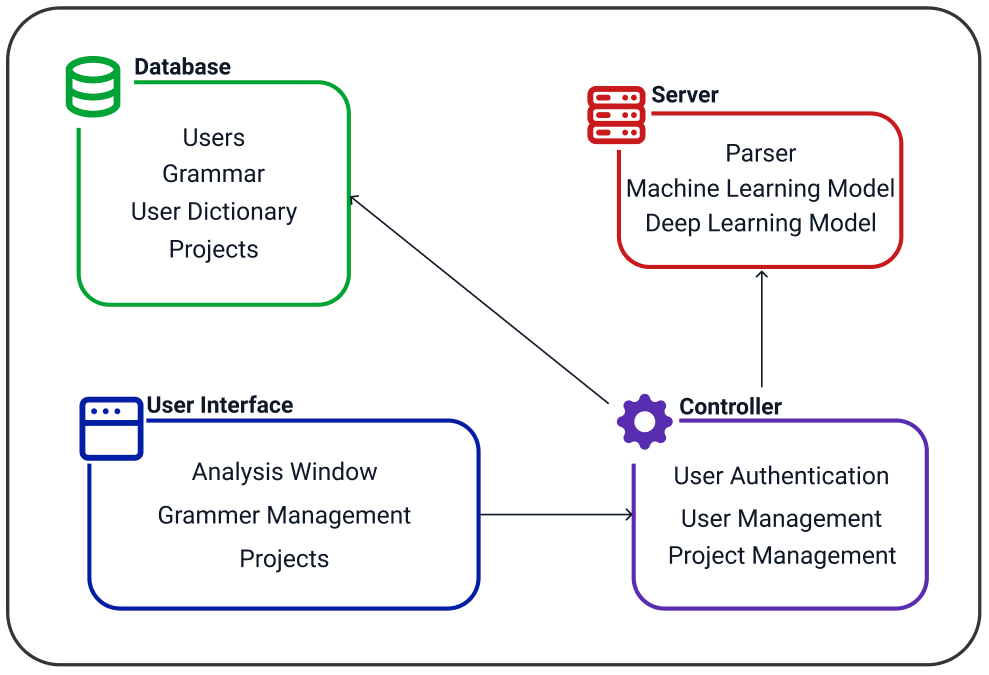
\includegraphics[width=0.7\linewidth]{images/System Overview.png}
    \caption{Architectural Design}
    \label{fig:image}
\end{figure}


\subsection{Decomposition Description}
\begin{figure}[H]
    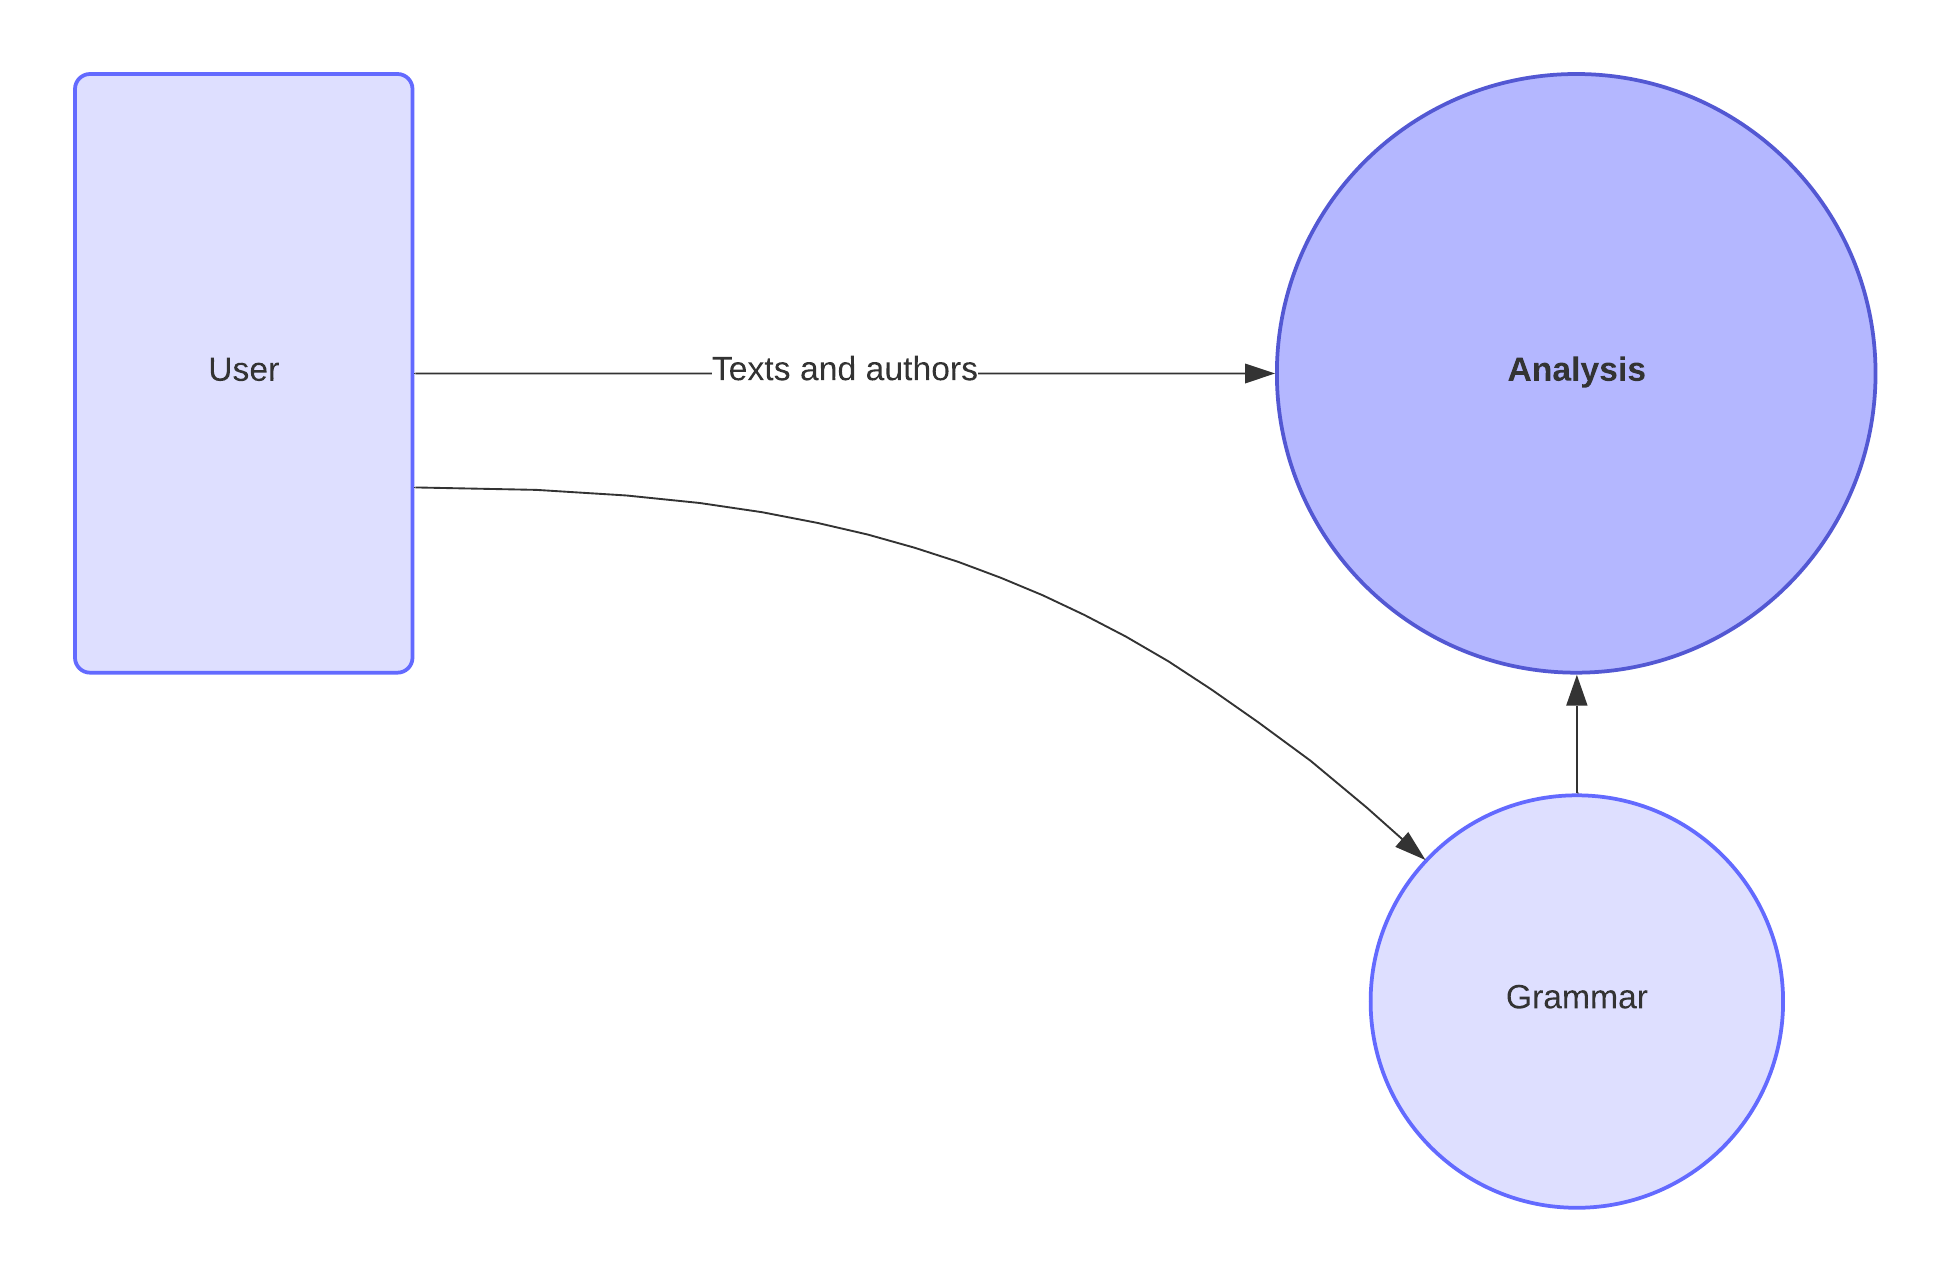
\includegraphics[width=15cm]{images/DFD.png}
    \caption{Data Flow Diagram}
\end{figure}

\begin{figure}[H]
    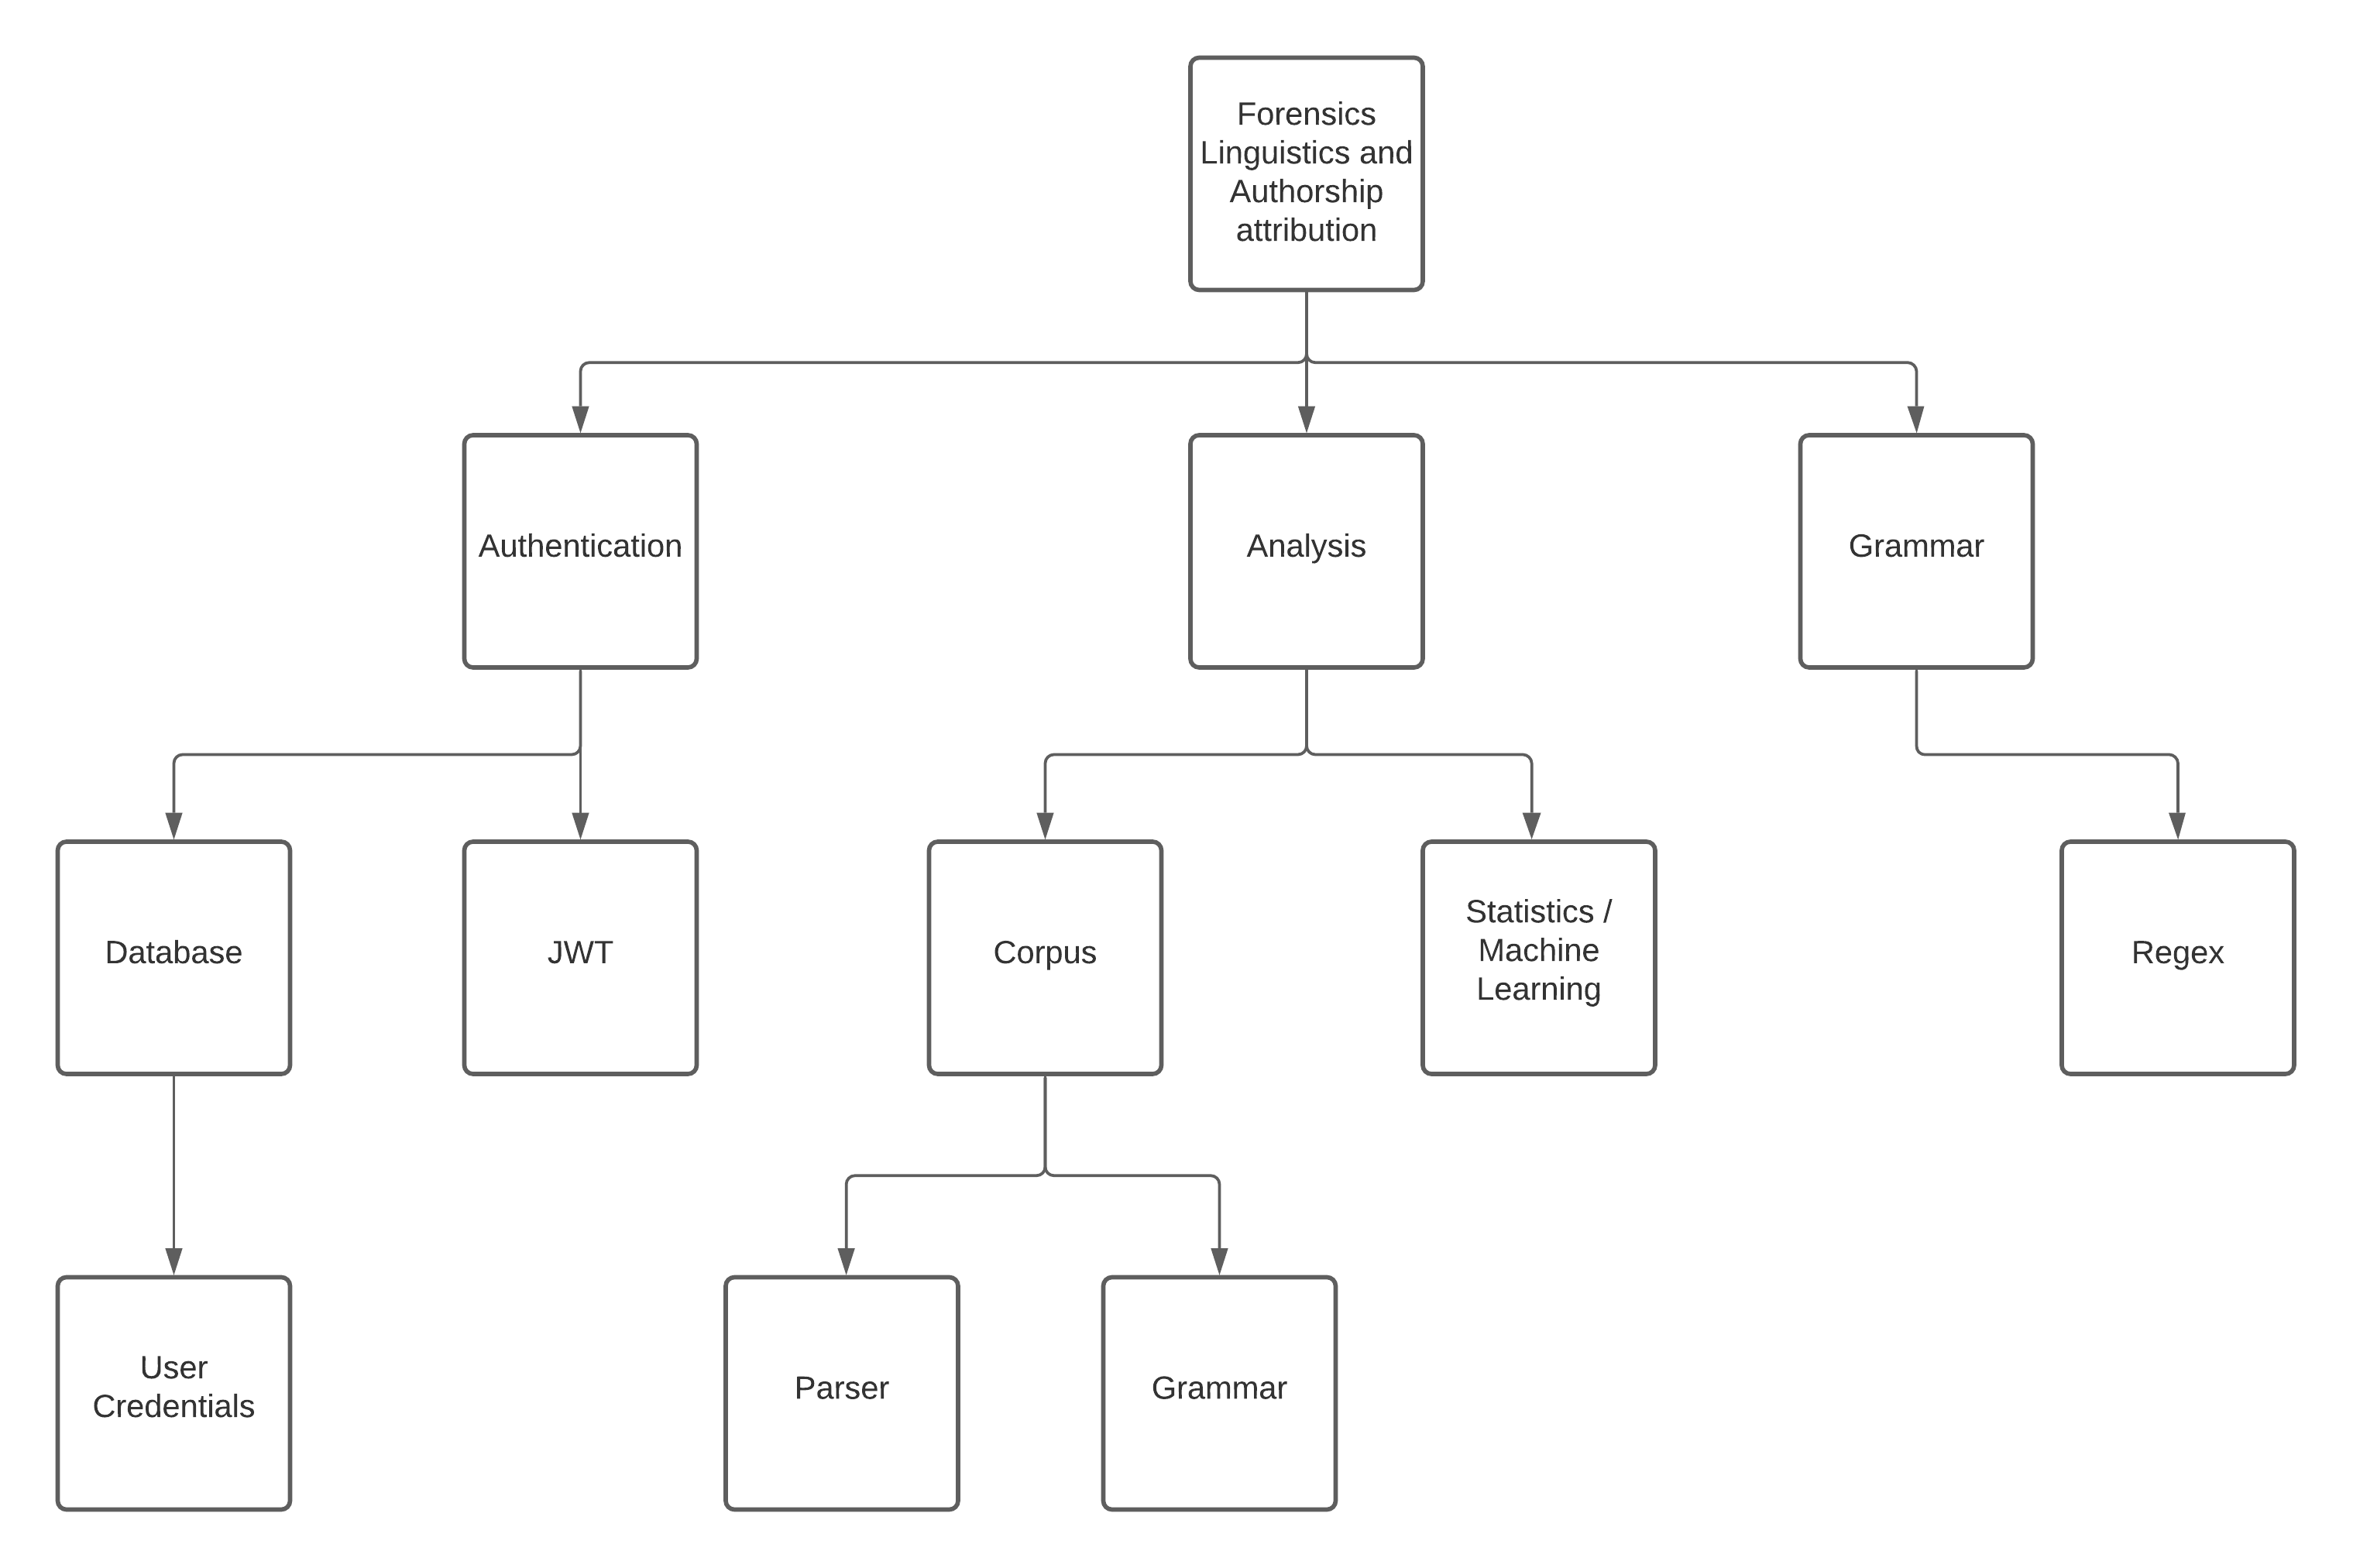
\includegraphics[width=15cm]{images/FDD.png}
    \caption{Functional Decomposition Diagram}
\end{figure}


\subsection{Design Rationale}
The principle behind the architecture used is separation of concerns, the main component of the system besides the user interface and the database is the server. The server, user interface, and database are completely separate entities that are deployed independently. The reason for the separation is that they use different technologies with different architectures and different deployment needs. The server hosts the text parser, which runs on python and has a very specific task that may be modified but no extra features may be added. The database exposes a graphQL API to query and manipulate the user data. The interface is the coordinator of all the processes of the system.


\section{Data Design}
\subsection{Data Description}
\begin{enumerate}
    \item Corpus \begin{itemize}
              \item The corpus is uploaded as a compressed file containing folders of the texts, with the authors being the title of each folder. The file is extracted and turned into JSON format before parsing, then each element of the JSON object is parsed and returned as a parsed array that is saved in a noSQL database completely dedicated to storing the corpus and their analysis results.
          \end{itemize}
    \item Grammar \begin{itemize}
              \item Grammar data is saved in a SQL database as a REGEX string that is imported during parsing of text, and editing of features. The grammar is created using a tool specifically made for this system.
          \end{itemize}
    \item Users \begin{itemize}
              \item User data is saved in a SQL database. The user data includes their credentials, projects, and grammar.
          \end{itemize}
    \item Projects \begin{itemize}
              \item Project data is split into multiple tables in a SQL database. The data includes collaborators, corpus id, and used features.
          \end{itemize}
\end{enumerate}

\subsection {Data Dictionary}

\begin{sortedlist}
    \sortitem{createGrammar(featureName: string, regex: string)}
    \sortitem{updateGrammar(featureId: number, regex: string)}
    \sortitem{uploadText(file: zip)}
    \sortitem{formatText(file: zip)}
    \sortitem{parse(corpus: \{[authorName]: string[][], \\ disputed: string[][]\}, grammar: string[])}
    \sortitem{updateAnalysis(wordIdx: number, featureId: number)}
\end{sortedlist}

\section{Component Design}

\subsection{Authentication}
\begin{verbatim}
  username = input(username)
  password = input(password)
  userId = Select userId from database 
                where username = username & password = password
  if userId
      response.send(userId, username, JWT) 
                // JWT Token is auto generated  
\end{verbatim}

\subsection{Analysis}
\begin{verbatim}
  corpus = input(corpus)
  grammar = input(grammar)
  formattedCorpus = format(corpus)
  parsedCorpus = parse(formattedCorpus, grammar)
  response.send(parsedCorpus)
\end{verbatim}

\subsection{Grammar}
\begin{verbatim}
  featureName = input(featureName)
  regex = input(regex)
  res.send(Insert Into database (featureName, regex),
   Values (featureName, regex))
\end{verbatim}

\section{Human Interface Design}

\subsection {Overview of User Interface}
\begin{itemize}
    \item Creating new grammar: The user will open the grammar tab and press on the 'New Feature' button, they will then be redirected to a page where they are presented with a tool that allows them to write the grammar which will be converted into regex for the parser.
    \item Editing grammar: On the grammar tab, the user will be presented with a list of all the features they created, which they can either delete or edit. If the user chooses to edit, they will be redirected to the grammar creation tool page, but with the existing feature characteristics already set for them to change.
    \item Creating a project: The user will be presented with a wizard involving a number of steps, they will first upload the corpus in a specified format which will be demonstrated on the wizard, then they will choose the needed features from the grammar they created, or use one from the community, then all the data will be sent to the server and the user will be redirected to the workspace page where they can see the result of the analysis.
    \item Editing the analysis: The user can hover on any word in the workspace, set as a feature or not, and change its feature association as they please by selecting from the list of features they chose at the beginning of the project. The edit will also reflect on the statistical and the authorship attribution results accordingly.
\end{itemize}

\subsection {Screen Images}
\begin{figure}[H]
    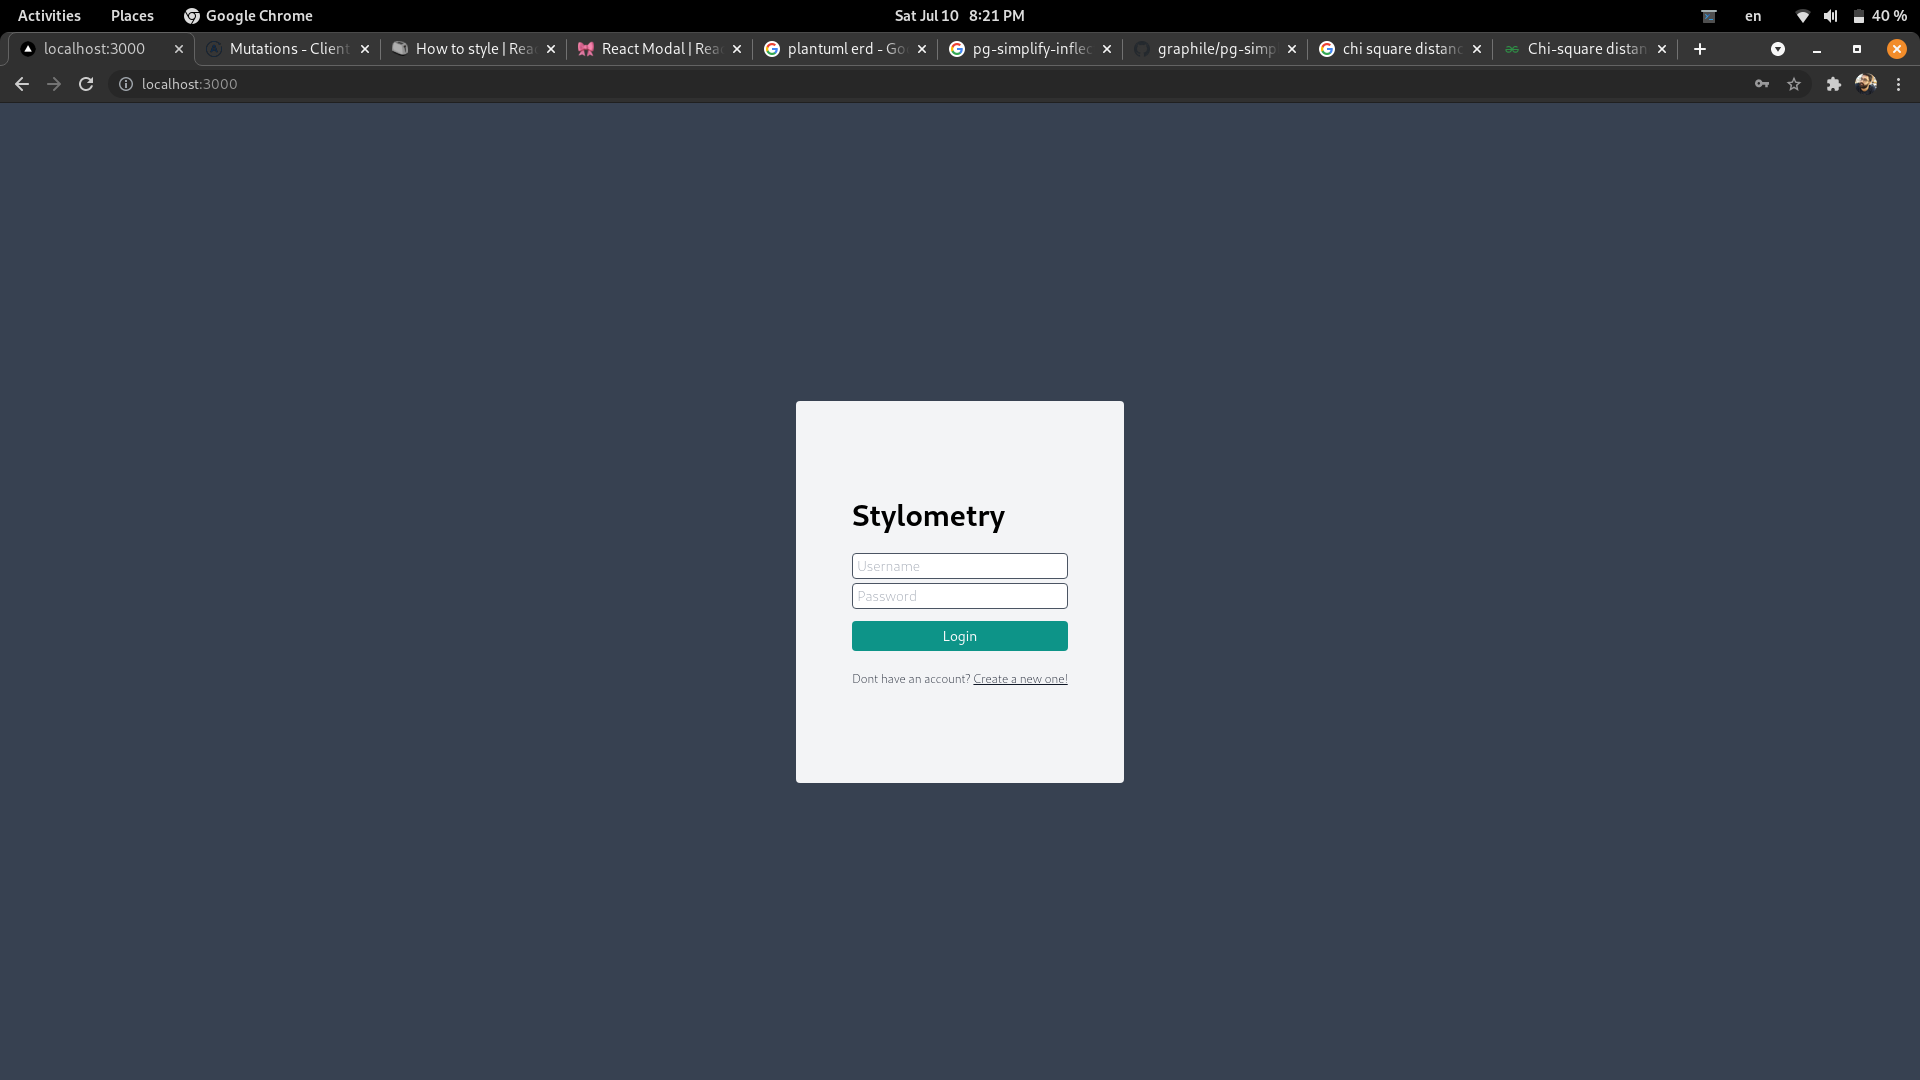
\includegraphics[width=15cm]{images/Login.png}
    \caption{Login}
\end{figure}

\begin{figure}[H]
    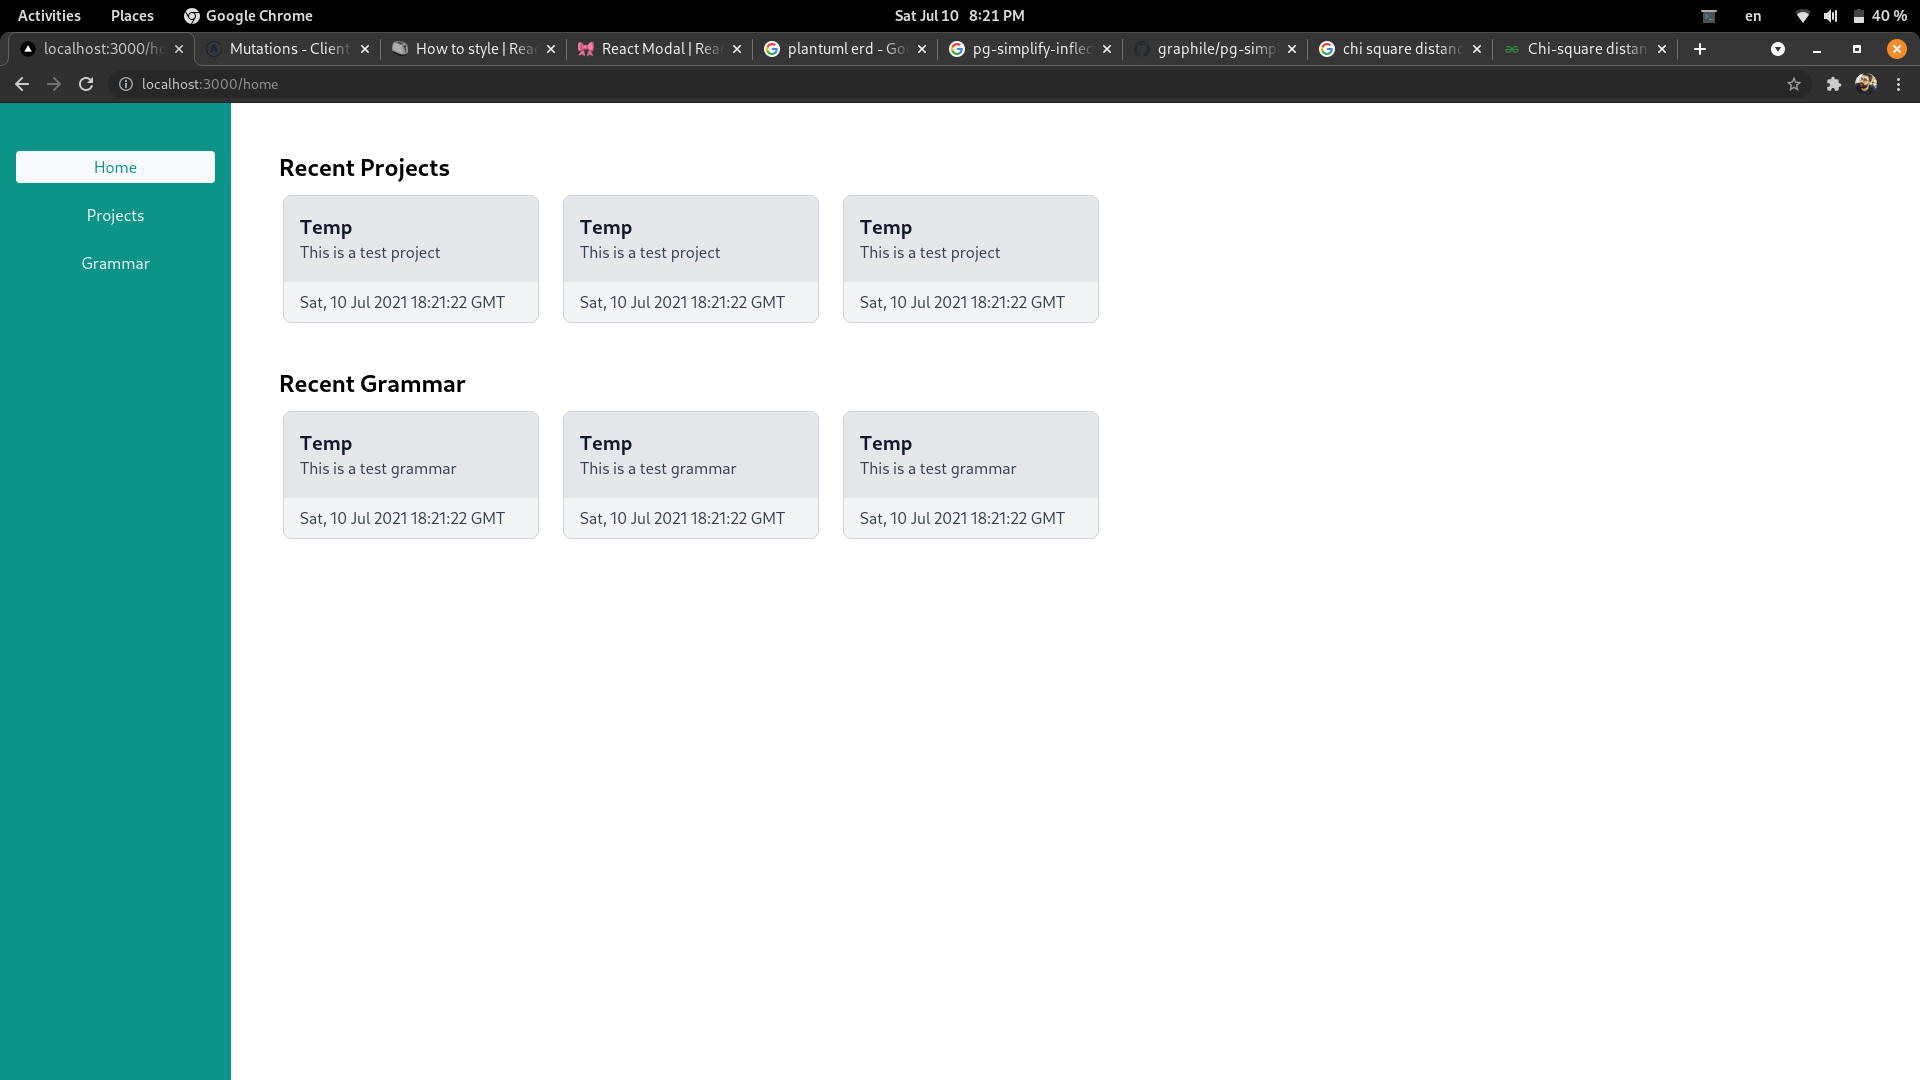
\includegraphics[width=15cm]{images/Home.png}
    \caption{Home}
\end{figure}

\begin{figure}[H]
    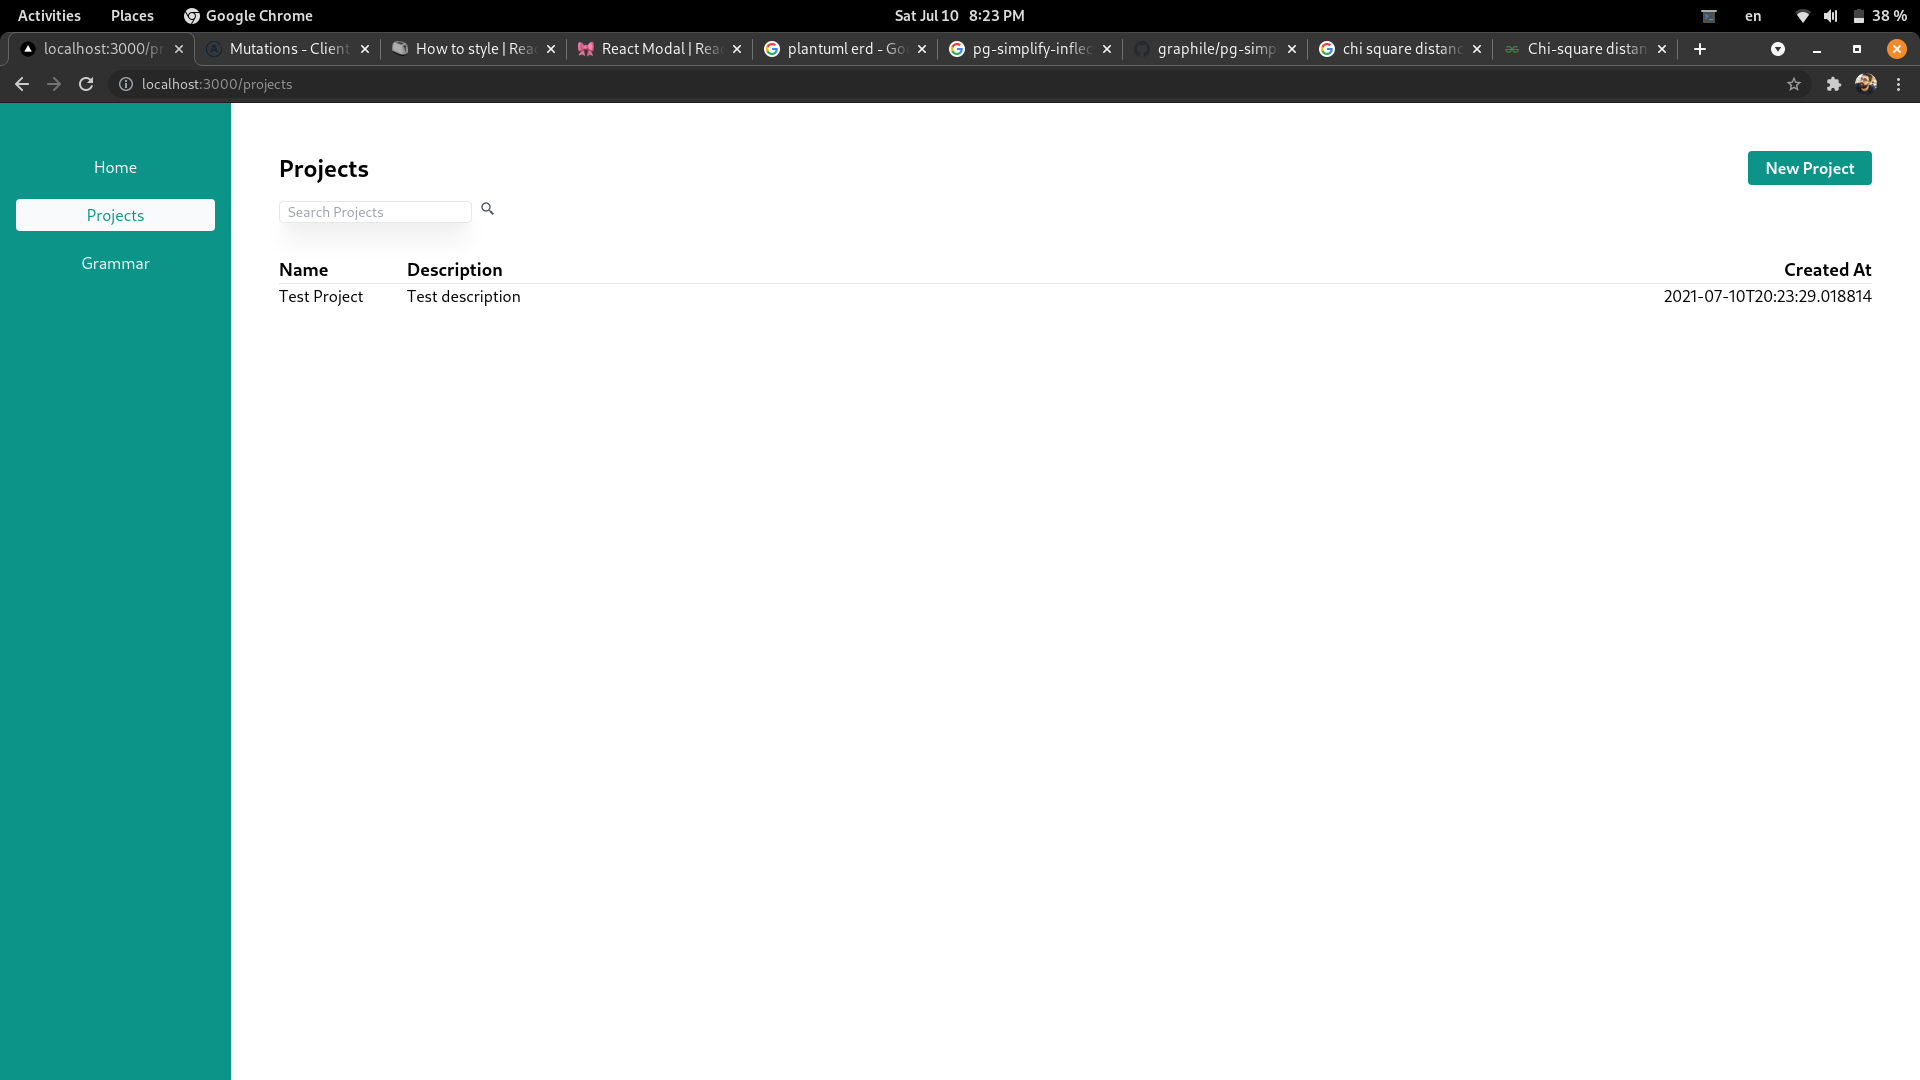
\includegraphics[width=15cm]{images/Projects.png}
    \caption{Projects}
\end{figure}
\begin{figure}[H]
    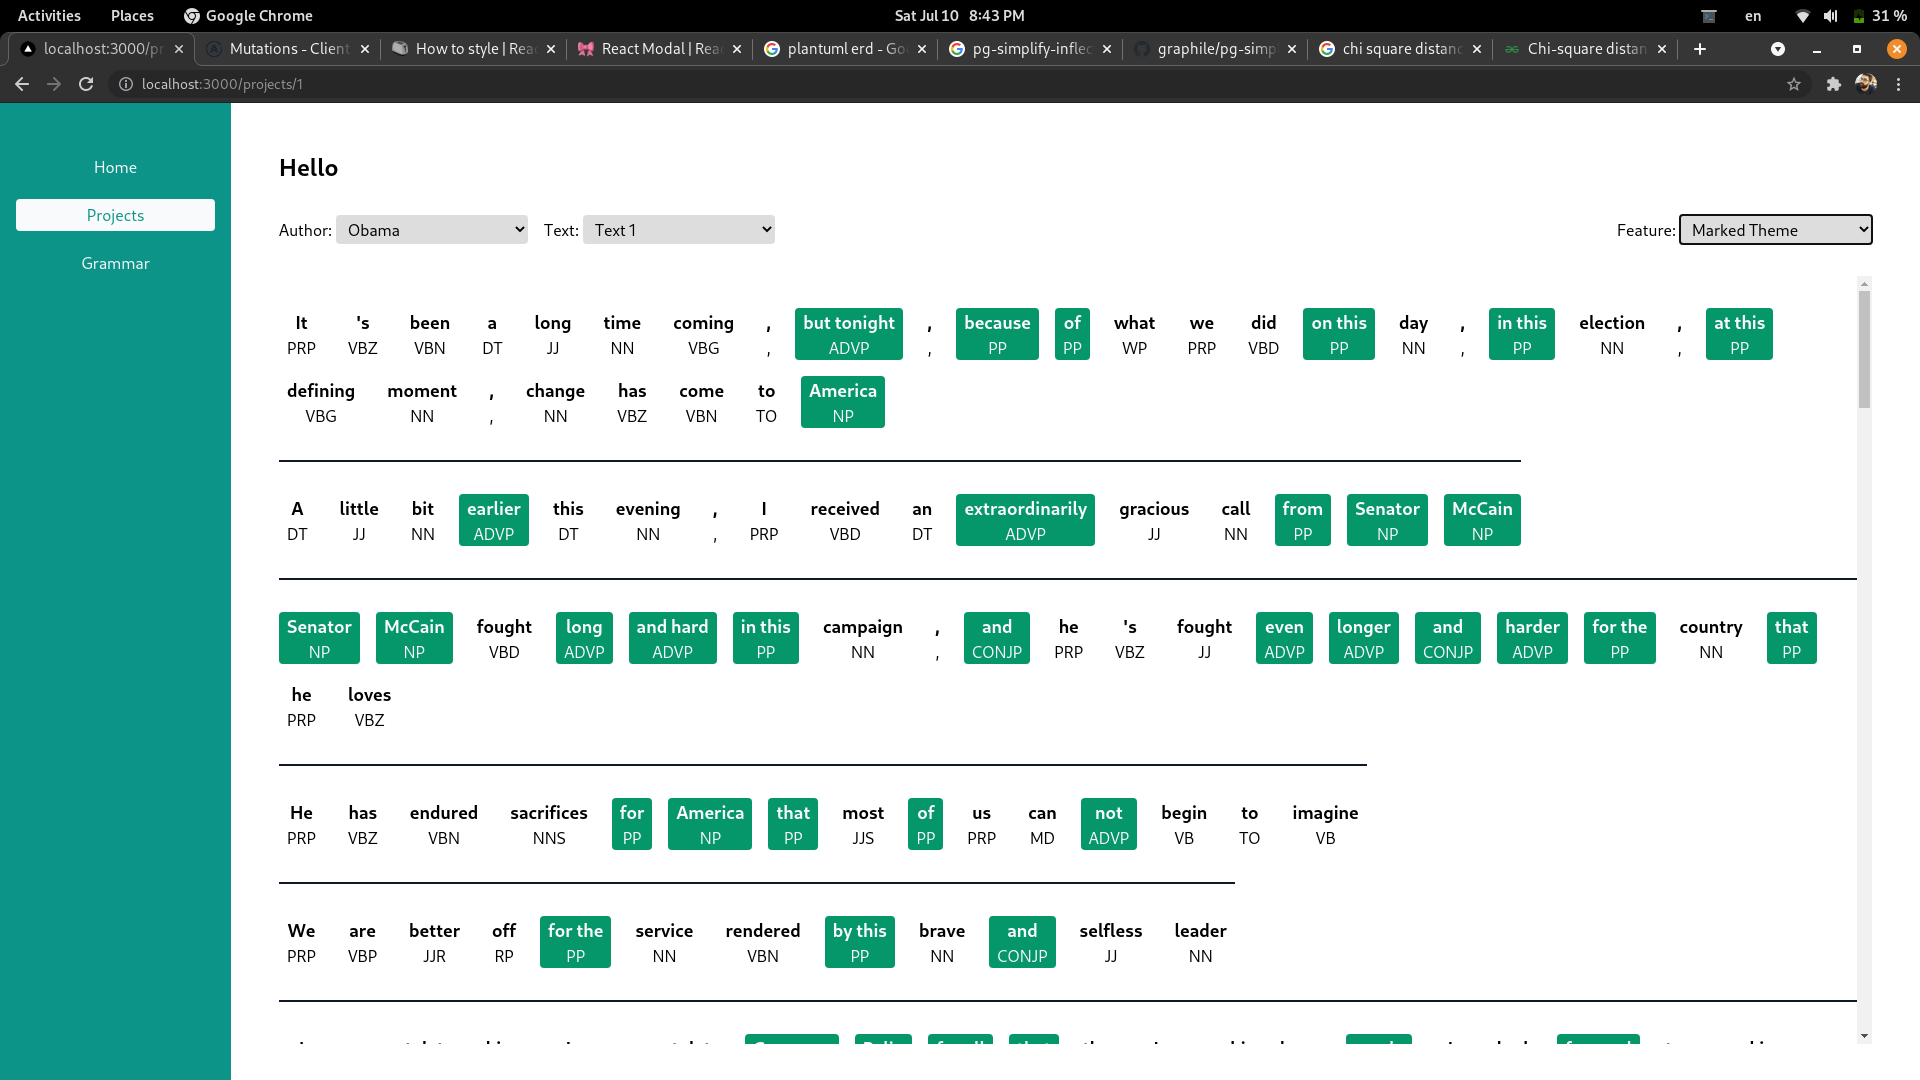
\includegraphics[width=15cm]{images/Project.png}
    \caption{Project}
\end{figure}

\begin{figure}[H]
    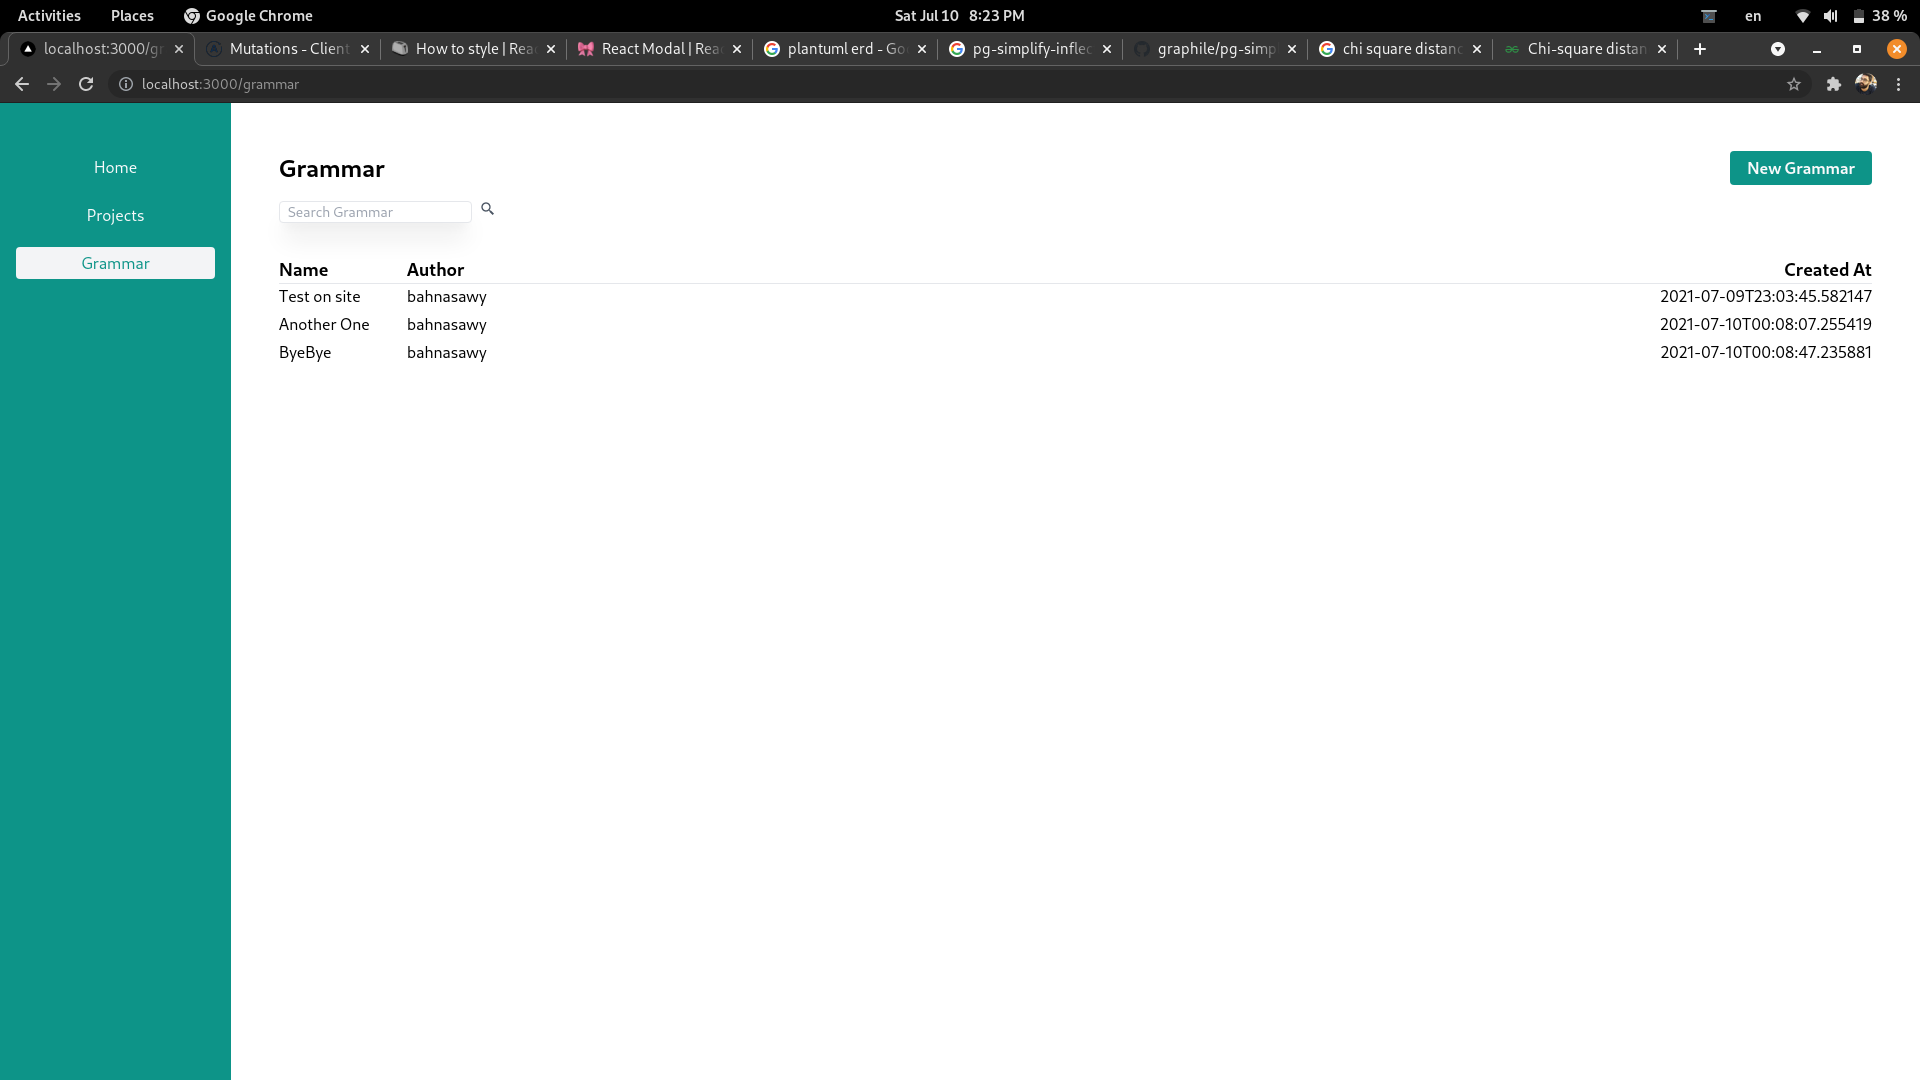
\includegraphics[width=15cm]{images/Grammars.png}
    \caption{Grammars}
\end{figure}

\begin{figure}[H]
    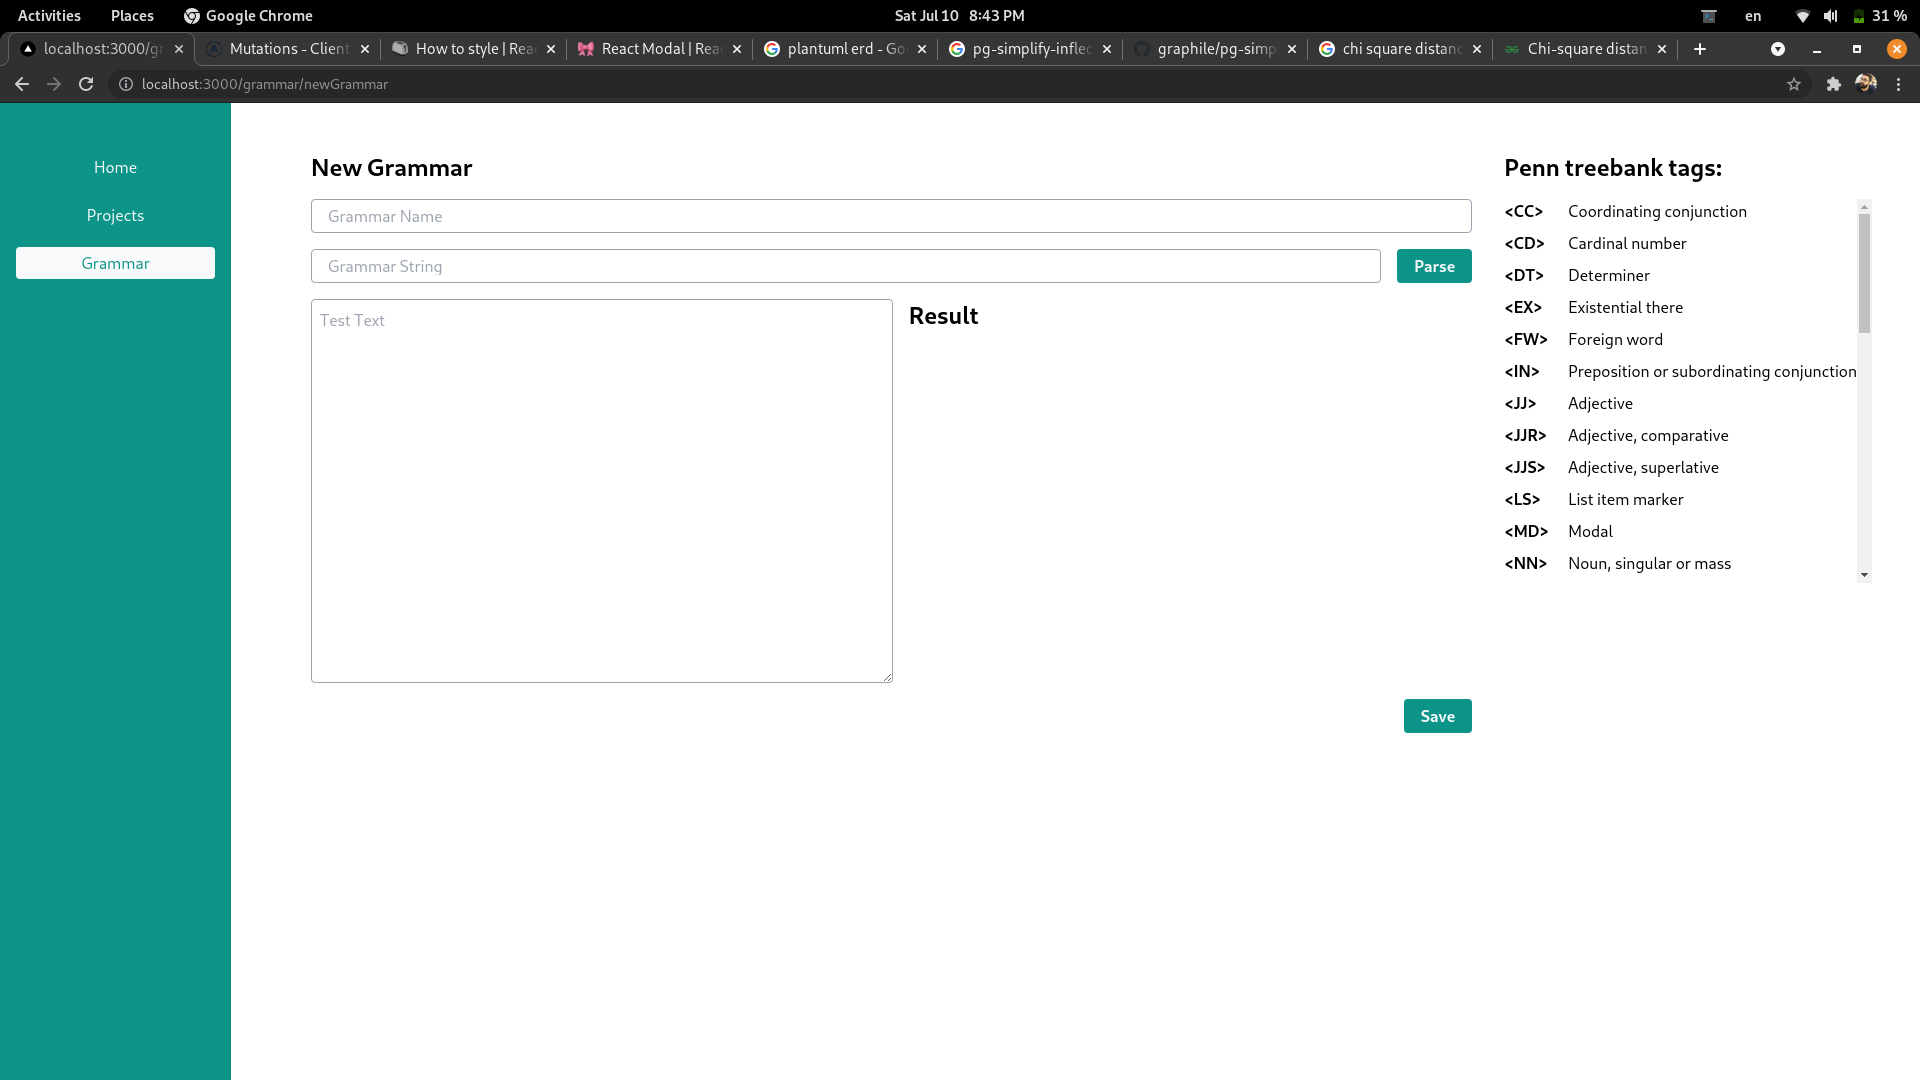
\includegraphics[width=15cm]{images/Grammar.png}
    \caption{Grammar}
\end{figure}


\section{Requirements Matrix}
\begin{center}
    \begin{tabular}{|c|c|}
        \hline
        System Components & Functional Requirements \\
        \hline\hline
        Grammar           & 3, 4                    \\
        \hline
        Analysis          & 1, 2, 5, 6, 7, 8        \\
        \hline
        Authentication    & 9, 10, 11               \\
        \hline
    \end{tabular}
\end{center}
